\section{A Quadratic Trajectory Function (Day 2)}

\myCenteredBox[width=5in]{
    Today you will 
    \begin{itemize}[nosep,label=\checkmark]
        \item Launch \mymm{}s from your catapult.
        \item Time and measure the \mymm~trajectories.
        \item Find a quadratic function that describes the trajectories.
    \end{itemize}
}

Here is the general idea.
\begin{itemize}[nosep]
    \item You will launch your \mymm{}s from your catapult.
    \item The candy will fly across the room following a parabolic trajectory.
\end{itemize}

\begin{center}
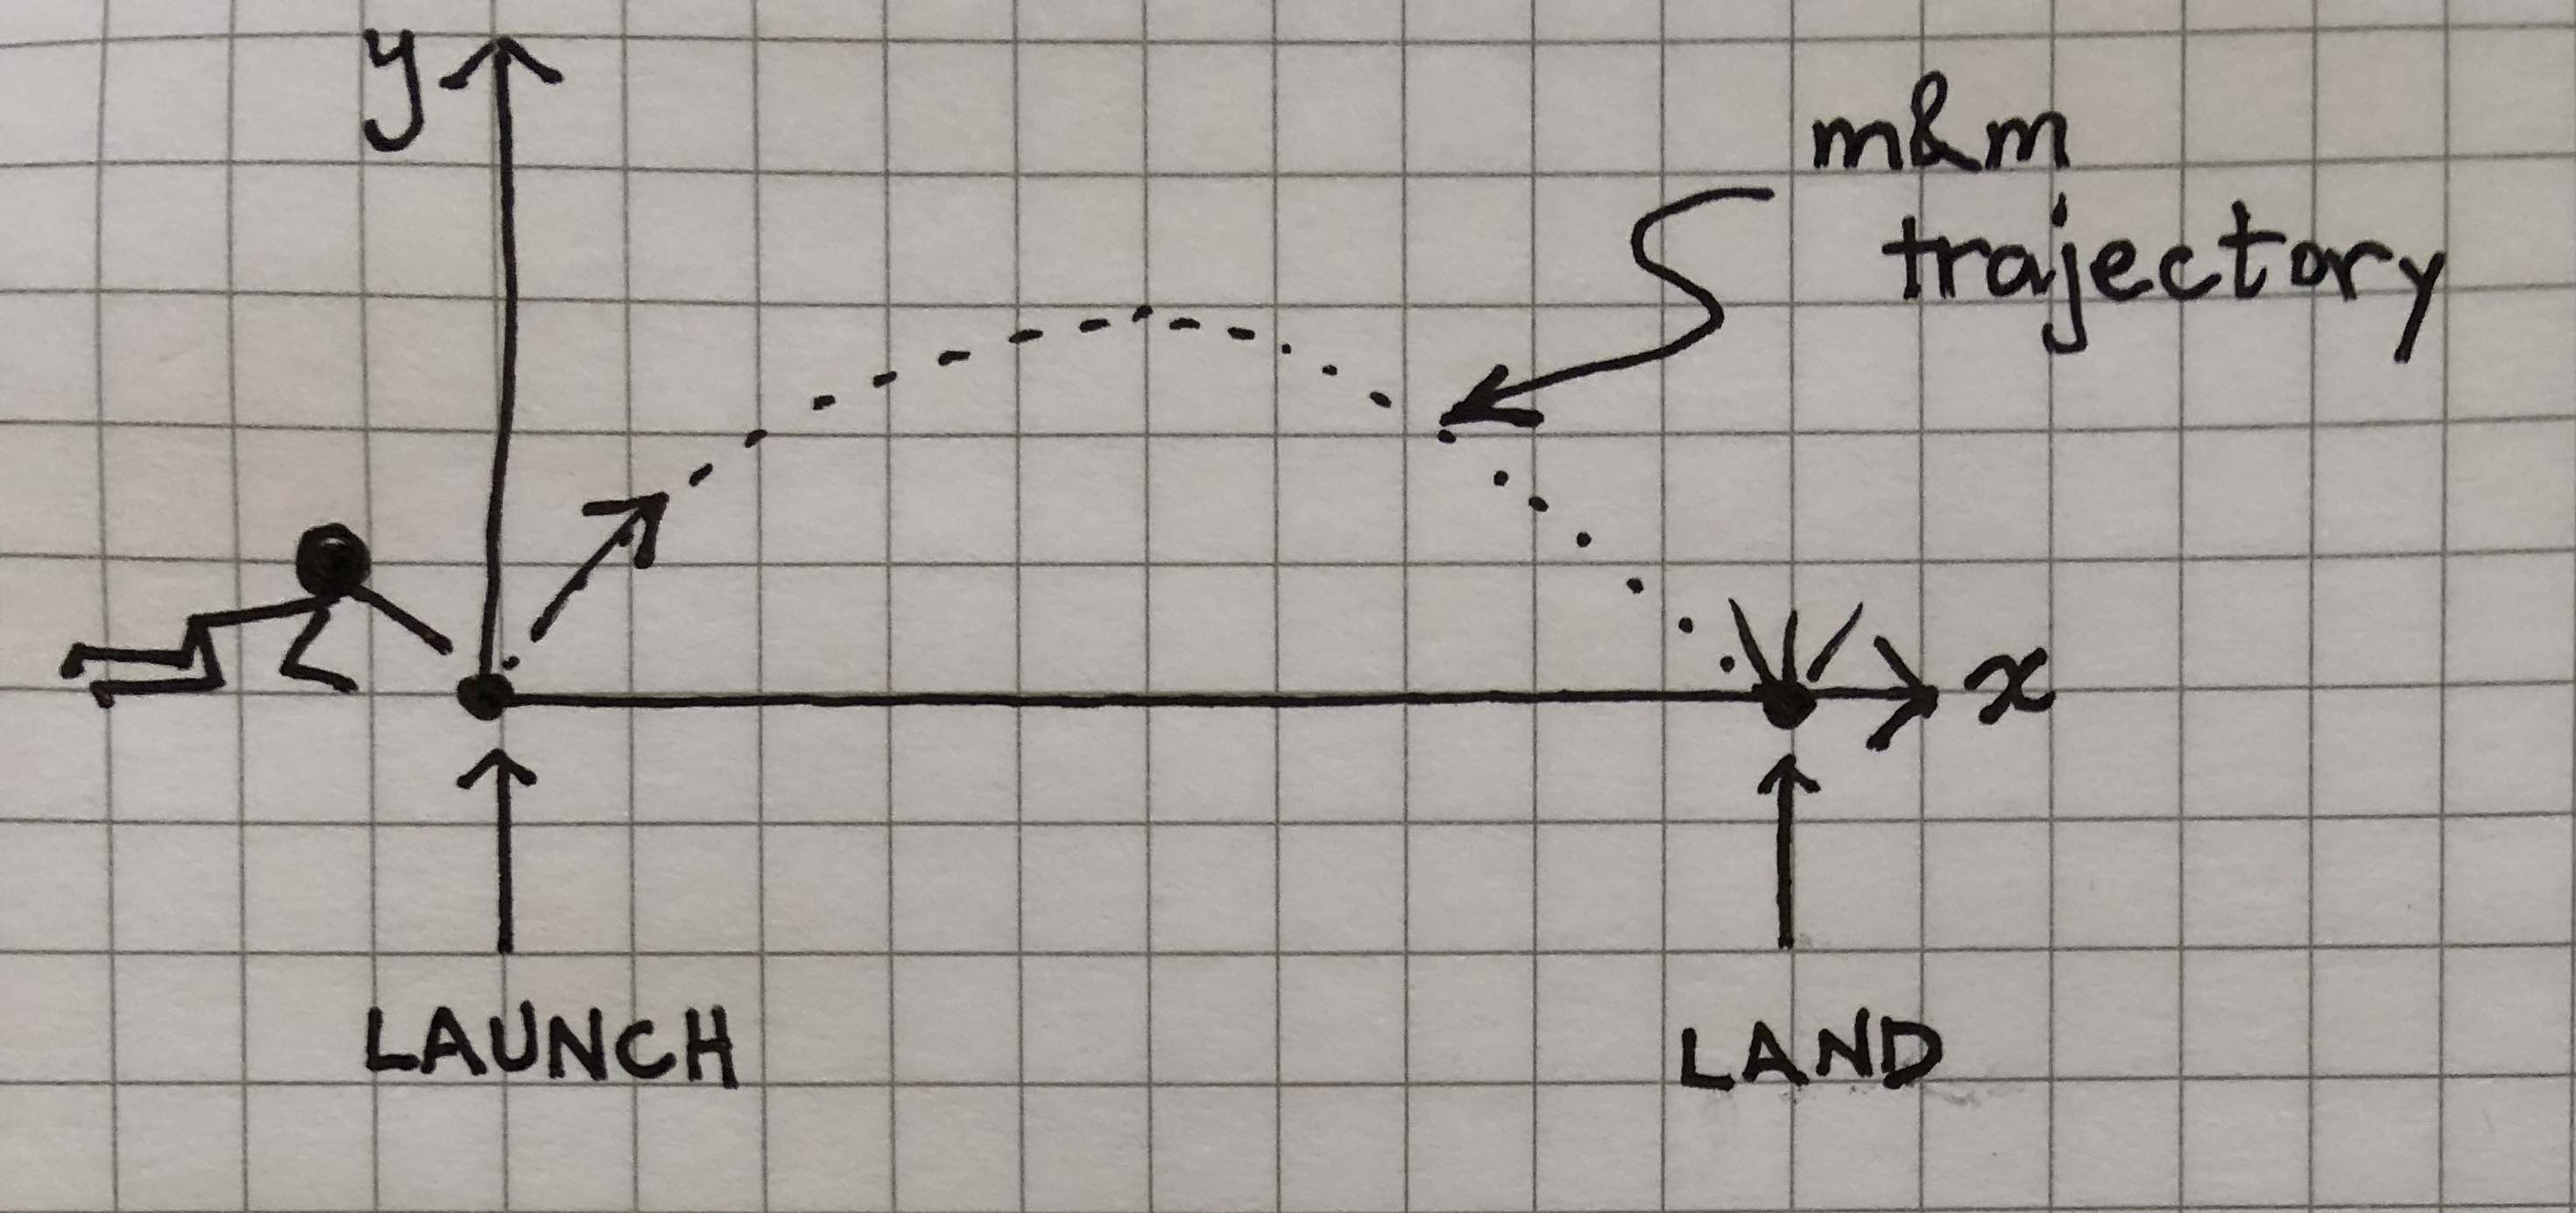
\includegraphics[width=3in]{../launch-and-landing.jpg}
\end{center}